% Draft report in the IEEE conference format (IEEEtran class, CTAN: ctan.org/pkg/ieeetran).
% Compile with: pdflatex main && bibtex main && pdflatex main && pdflatex main  (or upload the folder to Overleaf)
% Everything marked TODO in red still needs input or results.
\documentclass[conference]{IEEEtran}

\usepackage{graphicx}
\usepackage{booktabs}
\usepackage{amsmath}
\usepackage{xcolor}
\usepackage{tikz}
\usetikzlibrary{arrows.meta, positioning}
\usepackage{url}

\newcommand{\todo}[1]{\textcolor{red}{[TODO: #1]}}

\begin{document}

\title{When to Ask the Server: Adaptive Mask Refresh for Asynchronous Edge--Server Video Segmentation}

\author{\IEEEauthorblockN{Mykyta Voievudskyi}
\IEEEauthorblockA{\todo{institute, university}\\
\todo{city, country}\\
\todo{e-mail}}}

\maketitle

\begin{abstract}
A client that sees a video stream but cannot run a segmentation model itself has to ask a server for masks. The answers arrive late and cost bandwidth, so the client segments only some frames and has to keep useful masks in between. We study this setting on the KITTI MOTS development sequences with a YOLO segmentation model on a GPU server and dense optical flow on the client. Optical-flow propagation keeps most of the accuracy when refreshing every 5th frame (IoU 0.84 against 0.90 for segmenting every frame), and the delay of the server hurts only by making the shown masks older. We then let the client decide when to refresh, with a maximum mask age and a trigger based on the residual of the flow-warped previous frame around the mask boundary. On a fast connection the boundary residual gives 0.014 to 0.020 higher IoU than fixed intervals at the same request rate, about 10\,\% fewer requests for the same accuracy, but this effect is of the same size as the variation of the real latency between runs. On a simulated 2\,Mbit/s uplink the residual trigger adds no measurable benefit, while limiting the client to one outstanding request turns the worst fixed policy (IoU 0.45) into the best one (0.63). \todo{update with the controlled rerun and held-out results}
\end{abstract}

\begin{IEEEkeywords}
video segmentation, edge computing, computation offloading, optical flow, keyframe scheduling
\end{IEEEkeywords}

\section{Introduction}

Many devices that observe the world through a camera, such as vehicles, robots or phones, cannot run a modern segmentation network on every frame. A common way out is to send frames to a server with a GPU. This brings two costs. Every request uses uplink bandwidth, and the answer arrives only after the network and the server have done their part, so the mask describes a frame the client has already left behind.

The client can therefore not show a fresh segmentation on every frame. It has to keep a mask between the answers of the server, and it has to decide which frames to send. This report studies both parts on driving video:

\begin{enumerate}
\item How much accuracy is lost when segmentation runs only every $N$ frames, and how much of it does optical-flow propagation on the client recover?
\item How does the server's delay affect this?
\item Can a rule that uses only information available on the client decide when to refresh better than a fixed interval, at the same number of requests?
\item How do these policies behave on a slow, limited uplink?
\end{enumerate}

The contributions are an asynchronous client--server setup with a real GPU server, an evaluation of hold and flow propagation under delay, a residual-based refresh trigger evaluated against fixed intervals at matched request rates, and the observation that on a limited uplink the limit on outstanding requests matters far more than the trigger.

\section{Related Work}

\textbf{Keyframe propagation in video segmentation.} Running a heavy network only on keyframes and propagating results in between is well established. Deep Feature Flow~\cite{zhu2017dff} propagates network features with optical flow, and Clockwork Convnets~\cite{shelhamer2016clockwork} update parts of a network at different rates. Adaptive keyframe scheduling chooses keyframes from low-level feature changes~\cite{li2018lowlatency} or from a learned estimate of the expected accuracy~\cite{xu2018dvsnet}. These works run on one machine, without network delay and without bandwidth limits.

\textbf{Offloading from mobile devices.} Glimpse~\cite{chen2015glimpse} sends frames to a server for recognition only when the scene changes and tracks objects locally in between, which is closest to the setting here. Liu et al.~\cite{liu2019edgear} reduce the latency of edge-assisted detection for augmented reality by parallelising streaming and inference and by tracking on the device. \todo{read and summarise one or two more recent offloading papers}

This work combines the two lines in a simple, explainable form: propagation with classical dense optical flow, a refresh rule from the flow residual, and an evaluation that compares policies at equal request rates and includes a limited uplink.

\section{System}

\begin{figure}[t]
\centering
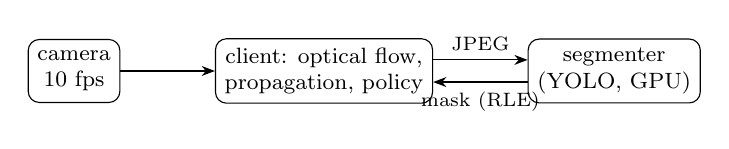
\begin{tikzpicture}[node distance=0.6cm and 1.2cm, box/.style={draw, rounded corners, align=center, font=\footnotesize, minimum height=0.8cm}, >={Stealth}]
\node[box] (cam) {camera\\10 fps};
\node[box, right=of cam] (client) {client: optical flow,\\propagation, policy};
\node[box, right=of client] (server) {segmenter\\(YOLO, GPU)};
\draw[->] (cam) -- (client);
\draw[->] ([yshift=4pt]client.east) -- node[above, font=\scriptsize] {JPEG} ([yshift=4pt]server.west);
\draw[->] ([yshift=-4pt]server.west) -- node[below, font=\scriptsize] {mask (RLE)} ([yshift=-4pt]client.east);
\end{tikzpicture}
\caption{Setup. The client sends some frames and does not wait; masks arrive later and are moved to the current frame with optical flow.}
\label{fig:system}
\end{figure}

Fig.~\ref{fig:system} shows the setup. The client replays the frames at the recording rate of 10\,fps. When its policy decides to refresh, it encodes the current frame as JPEG (quality 90, about 137\,KB) and sends it to the segmenter without waiting for the answer. The segmenter runs a pretrained Ultralytics YOLO26m segmentation model~\cite{ultralytics} and returns the union of all \emph{person} and \emph{car} masks, compressed as run-length encoding (about 1\,KB).

\textbf{Propagation.} On every frame the client computes dense backward optical flow from the current to the previous frame with OpenCV DIS~\cite{kroeger2016dis} and moves the shown mask with it. When a mask arrives it describes an older frame, its source frame. The client moves it over all frames since then, using the flows it has already computed, so it never computes flow on old frames again. The alternative, used as a baseline, holds the last mask unchanged.

\textbf{Mask age.} The age of the shown mask is the number of frames between its source frame and the current frame. It is the main quantity that links delay and accuracy in the results.

\textbf{Deployment.} \todo{say which runs used which hardware}. The baselines and delay experiments ran the segmenter on the laptop GPU (RTX 4060 Laptop). The policy experiments ran it on an NVIDIA V100 in a SLURM job on a computing cluster, reached through an SSH tunnel, with the client on the laptop. The messages are authenticated with a shared key, because they contain serialised Python objects.

\section{Refresh Policies}
\label{sec:policies}

All policies decide on every frame whether to send the current frame. Three are compared.

\textbf{Fixed interval} sends every $N$-th frame.

\textbf{Maximum interval} sends when the shown mask is at least $K$ frames old. It also does not send while a request newer than the shown mask is on its way, at most 2 requests may be outstanding, and two requests are at least 3 frames apart.

\textbf{Residual} uses the same rules as the maximum interval with $K=30$, and additionally sends when a residual signal crosses a threshold.

\subsection{Residual signals}

The residual reuses the flow that the client computes anyway. The previous grayscale frame is warped onto the current frame with the backward flow, the mean brightness of each frame is subtracted, and the residual is the absolute difference per pixel, in gray levels. Pixels whose flow points outside the previous frame are ignored. Where the flow explains the image well the residual is small.

\textbf{Boundary residual.} The mean residual in a band of about 7\,px around the boundary of the propagated mask (dilation minus erosion), summed over the frames since the shown mask's source frame. Errors of a propagated mask occur at its boundary, so this signal should grow as the mask drifts.

\textbf{Tile fraction.} The image is divided into $32\times32$ tiles. The signal is the share of tiles without mask pixels whose mean residual is above 12 gray levels. It is meant to react to new objects, which the boundary signal cannot see.

Raw flow magnitude is not used, because in driving video the camera moves and the flow is large everywhere, even when propagation works well.

\section{Experimental Setup}

\textbf{Data.} KITTI MOTS~\cite{voigtlaender2019mots}, based on KITTI~\cite{geiger2012kitti}, with the standard split. The 12 training sequences (5{,}027 frames) are used for development and the choice of thresholds. The 9 validation sequences are held out for the final evaluation. Only the classes person and car are used, the classes annotated in KITTI MOTS.

\textbf{Metric.} The predicted and annotated masks of each frame are combined over all objects. The IoU is the sum of intersections over all frames divided by the sum of unions, with ignore regions excluded, so frames where both masks are empty do not count.

\textbf{Cost.} The request rate in requests per second. All requests have about the same size, so the upload bandwidth is proportional to it (2.1\,Mbit/s at 2 requests/s).

\textbf{Simulated slow network.} A simulated link in the client adds, on top of the real connection, a limited uplink of 2\,Mbit/s where requests queue behind each other, a fixed extra delay of 50\,ms, and a random half-normal extra delay with a standard deviation of 20\,ms and a fixed seed. Each client has its own simulated link, so runs can be done in parallel. The download is not limited.

\textbf{Real time.} All policy experiments run in real time at 10\,fps, so the client's processing time and the real latency are part of the measurement. The client needs about 18\,ms per frame including about 4\,ms for the residual signals, and no frame took longer than the 100\,ms frame period. \todo{name the laptop CPU}

\section{Results}

\subsection{Baselines: propagation recovers most of the accuracy}

\begin{figure}[t]
\centering
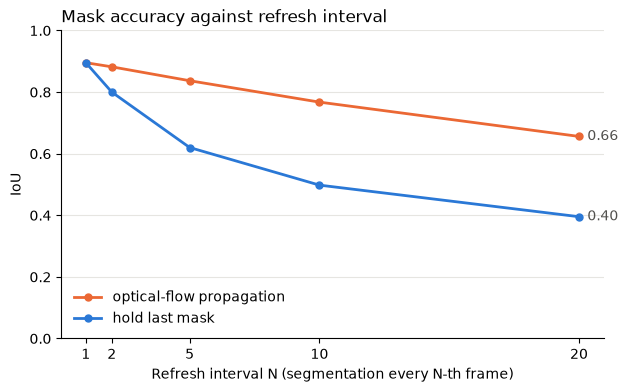
\includegraphics[width=\columnwidth]{figures/baselines_iou_interval.png}
\caption{IoU against refresh interval, without delay. Optical-flow propagation keeps most of the accuracy that is lost when holding the last mask.}
\label{fig:baselines}
\end{figure}

Segmenting every frame gives IoU 0.895, the best this model reaches on the data (Fig.~\ref{fig:baselines}). Holding the last mask loses accuracy fast, to 0.62 at $N=5$ and 0.40 at $N=20$. Flow propagation keeps 0.84 at $N=5$ and 0.66 at $N=20$, so it recovers about 80\,\% of the lost accuracy at $N=5$. Its typical error is a mask smeared over newly exposed background behind moving objects, where the flow has no correct match.

\subsection{Delay acts through the age of the mask}

With the client and the segmenter as separate processes and a controlled delay before a mask may be used, every 100\,ms of delay makes the shown masks one frame older on average. At $N=5$ the IoU with flow falls from 0.81 without added delay to 0.68 at 550\,ms, and with holding from 0.53 to 0.37. At equal mask age the IoU with and without delay differs by at most 0.003 for ages 1 to 4, so the delay costs accuracy only through the mask age.

\begin{figure}[t]
\centering
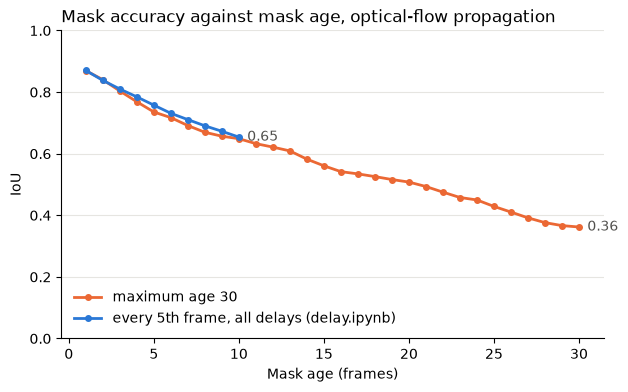
\includegraphics[width=\columnwidth]{figures/iou_mask_age.png}
\caption{IoU against mask age with flow propagation, from a run with a maximum mask age of 30 frames, and from the delay experiments.}
\label{fig:age}
\end{figure}

Fig.~\ref{fig:age} shows how far propagation carries a mask: from 0.87 at age 1 to 0.65 at age 10, 0.51 at age 20 and 0.36 at age 30.

\subsection{The residual signals carry information beyond the age}

From the run with a maximum age of 30, Fig.~\ref{fig:signals} compares masks of the same age: for each age, the rank correlation between a signal and the drop in IoU since the mask arrived. For young masks the summed boundary residual ranks the masks well (about 0.5 to 0.6 at ages 2 to 5), which is where a trigger has to decide. It weakens with age. The tile fraction is weaker but steady at about 0.2 to 0.3. Thresholds were then chosen from the distribution of the signals, at values the average mask reaches at ages of about 6, 11 and 17.

\begin{figure}[t]
\centering
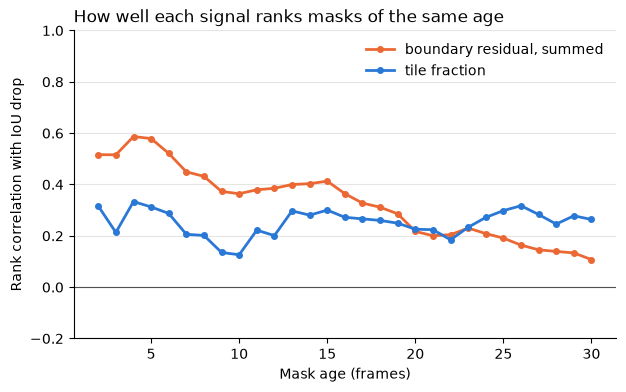
\includegraphics[width=\columnwidth]{figures/signal_rank_corr.png}
\caption{Rank correlation between each signal and the IoU drop since the mask arrived, computed separately for each mask age.}
\label{fig:signals}
\end{figure}

\subsection{Fast connection: a small gain from the boundary residual}

\begin{table}[t]
\centering
\caption{Fast connection, development sequences. Fixed intervals interpolated at the same request rate (log scale).}
\label{tab:fast}
\begin{tabular}{lcccc}
\toprule
Policy ($K=30$ plus) & req/s & IoU & fixed, same rate & gain \\
\midrule
boundary 60 & 1.39 & 0.785 & 0.771 & +0.014 \\
boundary 100 & 0.84 & 0.721 & 0.701 & +0.019 \\
boundary 150 & 0.58 & 0.646 & 0.626 & +0.020 \\
boundary 100 + tiles 0.45 & 0.89 & 0.723 & 0.711 & +0.012 \\
tiles 0.23 & 0.49 & 0.584 & 0.593 & $-0.009$ \\
tiles 0.45 & 0.38 & 0.552 & 0.562 & $-0.011$ \\
\bottomrule
\end{tabular}
\end{table}

On the fast connection a mask arrives one or two frames after its request (median 95\,ms). Fixed intervals give IoU 0.808, 0.739, 0.597 and 0.550 at 2.0, 1.0, 0.5 and 0.34 requests/s. The maximum-interval rule sends on exactly the same frames as a fixed interval in this setting, so it is not shown separately.

The boundary residual lies above the fixed curve at all three thresholds (Table~\ref{tab:fast}, Fig.~\ref{fig:fast}), by 0.014 to 0.020 IoU, which means fixed intervals need 9 to 13\,\% more requests for the same accuracy. The gain holds in 7 or 8 of the sequences that can be compared, but it is small per sequence. The tile fraction is worse than fixed intervals and mostly spends its requests on one sequence where much of the background is poorly explained by the flow, so it was dropped.

The share of masks used two frames instead of one frame after their request varied between runs from 14 to 37\,\%, depending on the load of the network and the cluster. One extra frame of age costs about 0.03 IoU for a young mask, so this variation is of the same size as the gain. The run with the largest gain had the most late masks, so the variation does not seem to cause the gain, but it makes the result uncertain. \todo{controlled rerun with a fixed delay of 150\,ms: confirm or reject the gain}

\begin{figure}[t]
\centering
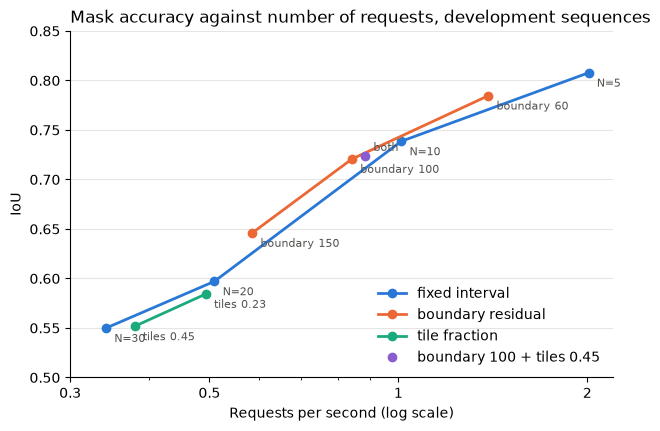
\includegraphics[width=\columnwidth]{figures/fast_requests_iou.png}
\caption{IoU against request rate on the fast connection.}
\label{fig:fast}
\end{figure}

\subsection{Slow uplink: the limit on outstanding requests matters most}

\begin{table}[t]
\centering
\caption{Simulated 2\,Mbit/s uplink with $50\pm20$\,ms extra delay. Boundary runs sum the residual from the mask's source frame.}
\label{tab:slow}
\begin{tabular}{lcccc}
\toprule
Policy & req/s & IoU & median latency & max.\ pending \\
\midrule
fixed $N=5$ & 2.01 & 0.447 & 1.67\,s & 17 \\
fixed $N=10$ & 1.01 & 0.607 & 0.70\,s & 2 \\
fixed $N=20$ & 0.51 & 0.524 & 0.70\,s & 1 \\
max.\ interval $K=5$ & 1.36 & 0.628 & 0.69\,s & 1 \\
max.\ interval $K=10$ & 1.01 & 0.607 & 0.70\,s & 1 \\
max.\ interval $K=20$ & 0.51 & 0.521 & 0.79\,s & 1 \\
boundary 60 & 1.05 & 0.613 & 0.69\,s & 1 \\
boundary 100 & 0.75 & 0.573 & 0.71\,s & 1 \\
boundary 150 & 0.53 & 0.527 & 0.70\,s & 1 \\
\bottomrule
\end{tabular}
\end{table}

On the simulated uplink, sending one frame takes about 0.55\,s and a mask is about 7 frames old when it arrives (Table~\ref{tab:slow}, Fig.~\ref{fig:slow}). Sending every 5th frame exceeds the capacity of the link. The requests queue up, the latency grows to more than 8\,s, and the IoU (0.45) falls below that of sending every 20th frame. The maximum-interval rule with $K=5$ wants the same refresh rate, but it does not send while a request is on its way. It therefore sends as soon as the previous answer is back, every 7.4 frames, uses the link exactly as much as it can carry without knowing its rate, and is the best policy (0.63).

The residual policy first sent much less than expected, because the boundary sum started when a mask \emph{arrived} rather than at its source frame, which ignores the 7 frames of drift during the transfer. With the sum from the source frame (the definition in Section~\ref{sec:policies}) it reacts earlier, but at the same request rate it is only 0.002 to 0.004 IoU above the maximum-interval rule and better in at most half of the sequences that can be compared, which is no measurable gain. When a mask is already old on arrival and a refresh cannot come faster than one round trip, there is little room left for choosing a better moment.

\begin{figure}[t]
\centering
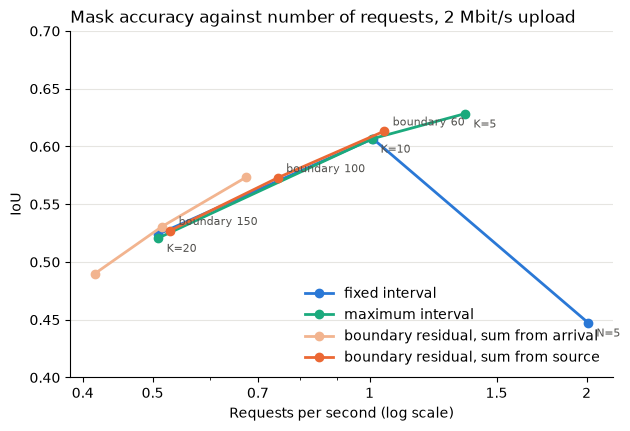
\includegraphics[width=\columnwidth]{figures/slow_requests_iou.png}
\caption{IoU against request rate on the simulated 2\,Mbit/s uplink. Fixed $N=5$ overloads the link.}
\label{fig:slow}
\end{figure}

\subsection{Held-out sequences}

\todo{evaluate the chosen settings on the 9 held-out sequences and report them here}

\section{Discussion and Limitations}

\todo{revise after the remaining runs}

The clearest result is not about the trigger. Flow propagation and a rule that keeps only one request in flight already give most of what a client can do, and on a limited uplink the second matters more than any choice of moment. The residual trigger is cheap (about 4\,ms per frame) and gives a small, uncertain gain on a fast connection.

The study has several limitations. Thresholds were tuned and compared on the same development sequences, and the held-out evaluation is still missing. Each setting was run once, and on the fast connection the real latency varied between runs. The slow network is simulated in the client and does not model a variable bandwidth, packet loss or a shared downlink. The masks of all objects are merged into one, so the evaluation does not see which objects are missed. Finally, frame selection was kept simple: the policy always sends the newest frame.

\section{Conclusion}

Optical-flow propagation lets a client segment only every 5th frame and keep IoU 0.84 instead of 0.90, and the delay of a remote server costs accuracy only by making masks older. A refresh trigger from the flow residual around the mask boundary gives a small gain over fixed intervals on a fast connection, which still has to be confirmed under controlled latency and on held-out data. On a slow uplink it adds nothing measurable, while a limit of one outstanding request turns the worst fixed policy into the best one. \todo{final numbers}

\bibliographystyle{IEEEtran}
\bibliography{refs}

\end{document}
